% \chapter{Measurement Results and Discussion}
\chapter{\DIFdelbegin \DIFdel{Měření}\DIFdelend \DIFaddbegin \DIFadd{Testování navrženého řešení}}
\DIFadd{Tato kapitola zahrnuje testování navržené gatewaye senzorové sítě viz. kapitola \ref{Návrh WSN}, napojené přes síť RS485 na infrastrukturu přístupového systému firmy IMA v univerzítní budově univerzity ČVUT za reálného provozu s připojenými koncovými zařízeními senzorové sítě}\DIFaddend , \DIFdelbegin \DIFdel{výsledky }\DIFdelend \DIFaddbegin \DIFadd{které souběžně odesílají data. Ze zachyceného provozu dat v síti RS485 je odhadnut maximální počet připojených koncových zařízení souběžně odesílající data v senzorové síti při zachování správné funkce přístupového systému.
}

\DIFadd{Testování je provedeno v jednom bloku patra univerzity, kde je do jednoho kontrolního panelu připojeno dvanáct CKP zařízení přes síť RS485. Každé z nich ovládá jedny dveře, tedy jednu čtečku }\DIFaddend a \DIFdelbegin \DIFdel{diskuse}%DIFDELCMD < }
%DIFDELCMD < %%%
\DIFdelend \DIFaddbegin \DIFadd{dveřní zámek.
Do této sítě RS485 je navíc připojena navržená gateway jako třinácté CKP zařízení.
K této navržené gatewayi senzorové sítě jsou připojena dvě koncová zařízení typu RHF1S001, dostupné na trhu, vyrbené firmou RisingHF, obsahující senzory teploty a vlhkosti. Pro tento test jsou nakonfigurovány k odesílání dat ze senzorů s intervalem 5 minut.
}

\DIFadd{Gateway a CKP zařízení jsou zapojena dle blokového schematu v obrázku \ref{fig:ACS architecture IMA with geteway}.
Konkrétní rozmístění stávajcích dvanácti CKP zařízení, gatewaye a dvou koncových zařízení senzorové sítě v testovaných prostorách budovy je zobrazeno v obrázku \ref{fig:CorridorFloorPlan}.
}\DIFaddend 

\begin{figure*}[!ht]
    \centering
    \DIFdelbeginFL %DIFDELCMD < \includegraphics[width=0.9\textwidth]{5patro}
%DIFDELCMD <     %%%
\DIFdelendFL \DIFaddbeginFL \includegraphics[width=1\textwidth]{5patro}
    \DIFaddendFL \caption{\DIFdelbeginFL \DIFdelFL{Location of sensor nodes and }\DIFdelendFL \DIFaddbeginFL \DIFaddFL{Rozmístění koncových zařízení sítě a zařízení }\DIFaddendFL CKP \DIFdelbeginFL \DIFdelFL{devices on the university floor}\DIFdelendFL \DIFaddbeginFL \DIFaddFL{v testovaných prostorách budovy}\DIFaddendFL }
    \label{fig:CorridorFloorPlan}
\end{figure*}

%DIF <  One floor block of university building is selected to perform the test. It is equipped with twelve CKP devices, each controlling one Door Lock and one Reader. One Gateway is added to the infrastructure, i.e., thirteen devices are connected to one RS485 network. Two temperature/humidity sensor nodes are wirelessly connected to the Gateway. The Gateway and CKP devices are connected via RS485 network as shown in Fig. \ref{fig:Access control system architecture}. The specific location of CKP devices, Gateway and two sensor nodes on the floor is shown in Fig. \ref{fig:CorridorFloorPlan}.
\DIFaddbegin \DIFadd{Testování probíhalo od 21. září do 31. října, tedy v době přítomnosti studentů a zaměstnanců v testovaných prostorách. 
Po tuto dobu testování byly zaznamenávány přenášené pakety síti RS485, kontrolní panel přijal 1~876~978 paketů (14~074~522 B) a odeslal 1~101~556 paketů (8~295~219 B), dohromady tedy 2~978~534 paketů (22~369~741 B).
Z naměřených hodnot byla provedena metoda frekvenční analýzy. Z přenesených paketů byly nejdelší 3 o velikostí 40 bytů.
S ohledem na celkové množství paketů je to zanedbatelné množství, tj. 1,3E-04 \%.
Avšak vzhledem k povaze systému, tedy systému s primární funkcí řízení přístupu do omezených oblastí, se za nejhorší scénář považuje nepřekonatelný limit.
}\DIFaddend 

%DIF <  The long-term operation test is carried out from 21$^{st}$ September to 31$^{th}$ October, i.e., in the period involving the presence of students and employees in the classrooms and offices on the monitored floor of the university.
%DIF <  During this period, the Control Panel received 1~876~978 packets (14~074~522 Bytes) and sent 1~101~556 packets (8~295~219 Bytes) from/to RS485 network. 
%DIF <  The lengths of all 2~978~534 packets, i.e., 22~369~741 Bytes, are recorded in RS485 network during long-term operation test and the frequency analysis  method, i.e., the number of packet lengths in monitored period, is performed. Three packets reach the largest value, i.e., 40 Bytes. 
%DIF <  Considering the total amount of packets, it is negligible quantity, i.e, 1.3E-04\%. However, given the nature of the system, i.e., the system with the primary function of access to a restricted area, the worst-case scenario is considered to be an uncrossable limit. 
%DIF <  Number of sensor nodes that can be wirelessly connected to the Gateway and does not affect the existing access control system, can be calculated in dependence on used RS485 data rate. The reserve of the data rate is considered in order to protect the access control system from malfunction, e.g., a long waiting for the door to open.
\DIFaddbegin \DIFadd{Maximální počet koncových zařízení připojených ke gatewayi při kterém není ovlivněn stávájící přístupový systém je možné vypočítat z rychlosti přenosu dat v síti RS485. 
Tato rezerva rychlosti přenosu dat je uvažována za účelem ochrany přístupového systému před dysfunkcí nebo poruchou, například před dlouhým čekáním na otevření dveří.
}\DIFaddend 

%DIF <  \begin{table}[h]
%DIF <  \centering
%DIF <  \footnotesize
%DIF <  \caption{Packet length frequency analysis}
%DIF <  \begin{tabular}{cr}
%DIF <  Packet length &  Count \\ \hline
%DIF <  \textbf{7}  &  \textbf{2~216~098}  \\
%DIF <  8  &   619~127   \\
%DIF <  9  &         3   \\
%DIF <  11 &    58~393   \\
%DIF <  13 &    58~620   \\
%DIF <  16 &         1   \\
%DIF <  18 &         2   \\
%DIF <  \textbf{19} &    \textbf{26~286}   \\
%DIF <  23 &         1   \\
%DIF <  40 &         3   \\
%DIF <  \end{tabular}
%DIF <  \label{tab:FreqAnalysis}
%DIF <  \end{table}
\DIFaddbegin \begin{table}[h]
\centering
\footnotesize
\caption{\DIFaddFL{Frekvenční analýza délky paketu}}
\begin{ctucolortab}
    \begin{tabular}{|c|r|}
        \hline
\DIFaddFL{Packet length }&  \DIFaddFL{Count }\\ \hline
\textbf{\DIFaddFL{7}}  &  \textbf{\DIFaddFL{2~216~098}}  \\
\DIFaddFL{8  }&   \DIFaddFL{619~127   }\\
\DIFaddFL{9  }&         \DIFaddFL{3   }\\
\DIFaddFL{11 }&    \DIFaddFL{58~393   }\\
\DIFaddFL{13 }&    \DIFaddFL{58~620   }\\
\DIFaddFL{16 }&         \DIFaddFL{1   }\\
\DIFaddFL{18 }&         \DIFaddFL{2   }\\
\textbf{\DIFaddFL{19}} &    \textbf{\DIFaddFL{26~286}}   \\
\DIFaddFL{23 }&         \DIFaddFL{1   }\\
\DIFaddFL{40 }&         \DIFaddFL{3   }\\
\hline
\end{tabular}
\end{ctucolortab}
\label{tab:FreqAnalysis}
\end{table}
\DIFaddend 

%DIF <  \begin{figure*}[ht]
%DIF <      \centering
%DIF <      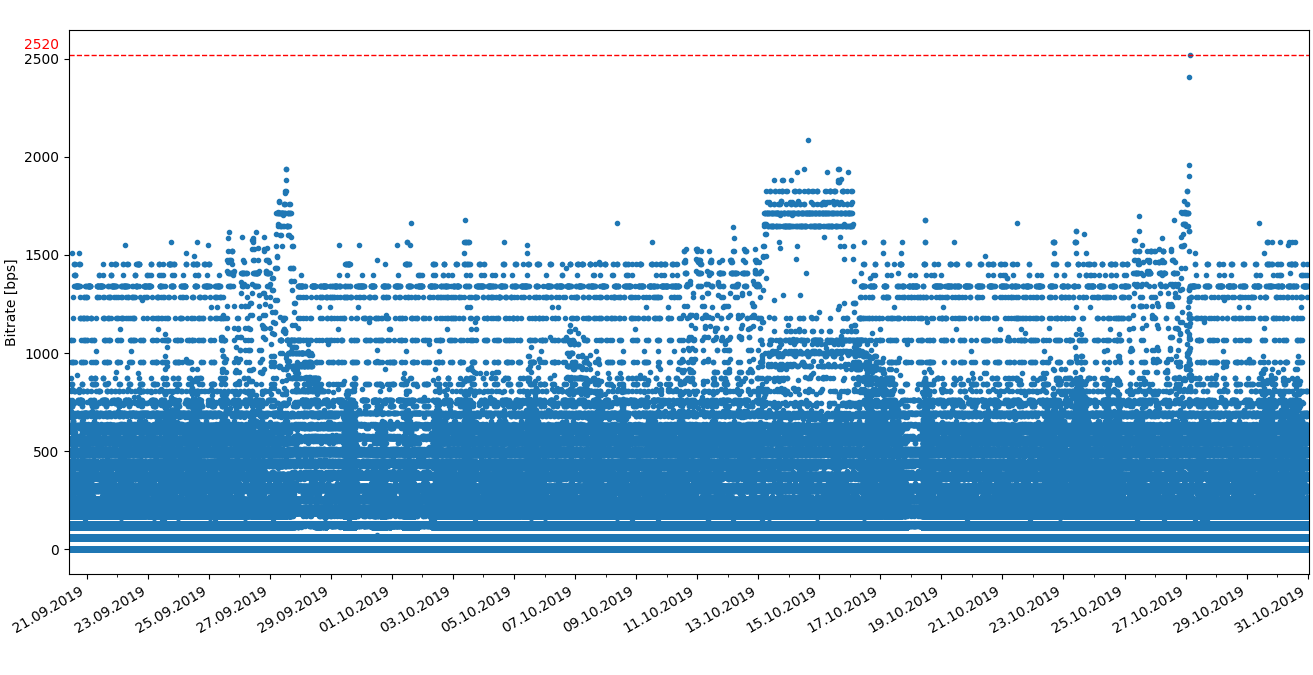
\includegraphics[width=1\textwidth]{03-dr-measured}
\DIFaddbegin \begin{figure*}[ht]
    \centering
    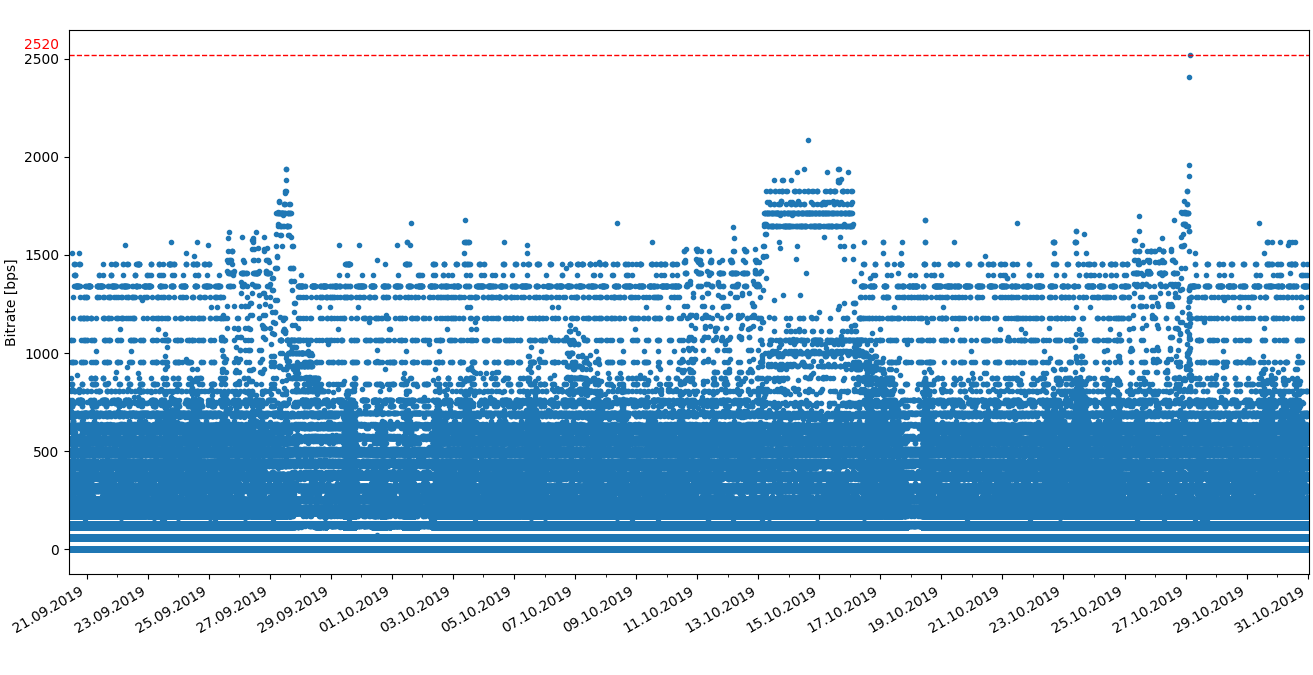
\includegraphics[width=1\textwidth]{03-dr-measured}
    \caption{\DIFaddFL{Měřená rychlost přenosu dat }[\DIFaddFL{bps}] \DIFaddFL{v síti RS485 během doby testování}}
    \DIFaddendFL % \caption{Measured data rate in [bps] in RS485 network during long-term operation test}
    %DIF <      \label{fig:PacketLengthMeasuredAll}
%DIF <  \end{figure*}
\DIFaddbeginFL \label{fig:PacketLengthMeasuredAll}
\end{figure*}
\DIFaddend 

%DIF <  Based on the frequency analysis given in Tab.~\ref{tab:FreqAnalysis} and IMA know-how, 19 Bytes length packets transmit sensor data, and 7 Bytes length packets are general aknowledgemets of IMA protocol. At least two packets are required to handle sensor data via RS485 network, i.e., one carrying sensor data and the other with ackowledgement.
\DIFaddbegin \DIFadd{Na základě frekvenční analýzy uvedené v tabulce \ref{tab:FreqAnalysis} a IMA know-how, pakety přenášející data z koncových zařízení jsou dlouhé 19 bytů a pakety potvrzení IMA protokolu jsou dlouhé 7 bytů. Alespoň dva pakety jsou potřeba k přenesení dat z koncových zařízení přes síť RS485, tj. paket s daty koncového zařízení a paket potvrzení.
}\DIFaddend 

%DIF <  %Fig. \ref{fig:PacketLengthMeasuredAll} shows 
%DIF <  %Two imporatnt characteristics are displayed, maximal length of packet (red colored dash line) and median length of packet (red colored solid line). It is determined by frequency analysis method as shown in Tab. \ref{tab:FreqAnalysis}. Average RS485 network channel traffic load is 6.38 pps, i.e., 0.85 Bps.
%DIF <  %shows lengths of captured packet  during
%DIF <  %Median of packet length is determined by using frequency analysis method, as shown in Tab. \ref{tab:FreqAnalysis}.
%DIF <  % 7,51 Byte --> simple arithmetic mean
\DIFaddbegin \DIFadd{V obrázku \ref{fig:PacketLengthMeasuredAll} jsou dvě důležité charakteristiky, maximální délka paketu 
(červená přerušovaná čára) a medián délky paketu (červená nepřerušovaná čára), určeny frekvenční analýzou v tabulce \ref{tab:FreqAnalysis}. 
Průměrné zatížení provozu kanálu sítě RS485 je 6,38 pps, tj. 0,85 Bps.
%DIF > shows lengths of captured packet  during
%DIF > Median of packet length is determined by using frequency analysis method, as shown in Tab. \ref{tab:FreqAnalysis}.
%DIF >  7,51 Byte --> simple arithmetic mean
}\DIFaddend 


%DIF <  During long term operation test, lengths of transmitted packets ($ l $) are captured with the accuracy of timestamps of a thousandth of a second. Then resampled to one second resolution interval using the sum function to easily represent achieved data as a bit rate in bit per second (bps),
%DIF <  Fig.~\ref{fig:PacketLengthMeasuredAll}.
%DIF <  Red colored dashed line (with value of 2520~bps) shows one second time interval in which a sum of captured packets is transported in RS485 network. It shows, based on detailed knowledge of the IMA protocol, less than 20\% of the RS485 network capacity is used. 
%DIF <  %This limit state is caused by data communication of two sensor nodes that occupied 2\% of capacity of used RS485 network.
\DIFaddbegin \DIFadd{Z testování provozu jsou zachyceny délky přenášených paketů ($ l $) s časovou přesností na tisícinu sekundy. Údaje o čase jsou převedeny na jednotky sekund pomocí funkce sum, aby byly získány data jako bitová rychlost v bitech za sekundu (bps),
V obrázku \ref{fig:PacketLengthMeasuredAll} červená přerušovaná čára s hodnotou 2520~bps) ukazuje jeden sekundový interval ve kterém součet přenesených paketů v síti RS485.
Na základě podrobných znalosti protokolu IMA se ukazuje, že je využito méně než 20\% kapacity sítě RS485 
%DIF > This limit state is caused by data communication of two sensor nodes that occupied 2\% of capacity of used RS485 network.
}\DIFaddend 

%DIF <  To avoid RS485 network congestion the maximum number of sensor nodes $ S_{MAX} $ can be calculated as:
%DIF <  \begin{equation}
%DIF <  S_{MAX} = \frac{\frac{\frac{v_{485}}{B}}{l_{MAX}} - R}{P}
%DIF <  \label{equ:max-count-of-sensors}
%DIF <  \end{equation}
\DIFaddbegin \DIFadd{Aby bylo zabráněno přetížení sítě RS485, maximální počet koncových zařízení připojených ke gatewayi $ S_{MAX} $ je možné vypočítat vztahem:
}\DIFaddend 

%DIF <  where:
\DIFaddbegin \begin{equation}
\DIFadd{S_{MAX} = \frac{\frac{\frac{v_{485}}{B}}{l_{MAX}} - R}{P}
\label{equ:max-count-of-sensors}
}\end{equation}
\DIFaddend 

%DIF <  \begin{tabular}{l @{  } l}
%DIF <  $v_{485}$ & 485 network data rate [bps]\\
%DIF <   B        & bits to Byte \\
%DIF <  $l_{MAX}$ & maximal packet length \\
%DIF <   R        & reserve of the data rate [\%]\\
%DIF <   P        & number of packets to transmit sensor data \\
%DIF <  \end{tabular}
\DIFaddbegin \DIFadd{kde:
}\DIFaddend 

%DIF <  Considering above mentioned limits, desired reserves and RS485 data rates, the maximum number of sensor nodes simultaneously transmitting their data on RS485 network is calculated, Tab. \ref{tab:max-sensor-nodes}.
\DIFaddbegin \begin{tabular}{l @{  } l}
\DIFadd{$v_{485}$ }& \DIFadd{rychlost přenosu dat v síti RS485 }[\DIFadd{bps}]\\
 \DIFadd{B        }& \DIFadd{počet bitů v bytu (pro přepočítání rychlosti přenosu dat na byty) }\\
\DIFadd{$l_{MAX}$ }& \DIFadd{maximální délka paketu }\\
 \DIFadd{R        }& \DIFadd{rezerva rychlosti přenosu dat }[\DIFadd{\%}]\\
 \DIFadd{P        }& \DIFadd{počt paketů k přenesení dat z koncového zařízení }\\
\end{tabular}
\DIFaddend 


%DIF <  Values for calculation are:
\DIFaddbegin \DIFadd{S ohledem na výše uvedené limity, navržené rezervy a rychlosti přenosu dat v síti RS485 je vypočítán maximální počet koncových zařízení senzorové sítě, které souběžně odesílají data přes síť RS485 viz. tabulka \ref{tab:max-sensor-nodes}.
}\DIFaddend 

%DIF <  \begin{tabular}{l @{ $=$ } l}
%DIF <  $v_{485}$ & RS485 network data rate \\
%DIF <   B        & 8 \\
%DIF <  $l_{MAX}$ & 40 \\
%DIF <   P        & 2 \\
%DIF <  \end{tabular}
\DIFaddbegin \DIFadd{Použité hodnoty pro výpočet jsou:
}\DIFaddend 

%DIF <  % todo: this table makes error
%DIF <  % \begin{table}[ht]
%DIF <  % \centering
%DIF <  % \footnotesize
%DIF <  % \caption{Maximum number of sensor nodes simultaneously transmitting their data in RS485 network with desired reserve}
%DIF <  % \begin{tabular}{r|rrrr}
%DIF <  % \multicolumn{1}{c|}{\textbf{RS485}}     & \multicolumn{4}{c}{\multirow{2}{*}{\textbf{Reserve} $R$}}\\
%DIF <  % \multicolumn{1}{c|}{\textbf{data rate}} &   \\
%DIF <  % $v_{485}$ {[bps]}  &	0 \%	&	10 \%	&	20 \%	&	30 \%  \\ \hline
%DIF <  %   1200~~~ &    1	&    1	&    1	&    1 \\
%DIF <  %   2400~~~ &    3	&    3	&    3	&    2 \\
%DIF <  %   4800~~~ &    7	&    6	&    6	&    5 \\
%DIF <  %   9600~~~ &   15	&   13	&   12	&   10 \\
%DIF <  %  19200~~~ &   30	&   27	&   24	&   21 \\
%DIF <  %  38400~~~ &   60	&   54	&   48	&   42 \\
%DIF <  %  57600~~~ &   90	&   81	&   72	&   63 \\
%DIF <  % 115200~~~ &  180	&  162	&  144	&  126 \\
%DIF <  % 230400~~~ &  360	&  324	&  288	&  252 \\
%DIF <  % 460800~~~ &  720	&  648	&  576	&  504 \\
%DIF <  % 921600~~~ & 1440	& 1296	& 1152	& 1008 \\
%DIF <  % \end{tabular}
%DIF <  % \label{tab:max-sensor-nodes}
%DIF <  % \end{table}
\DIFaddbegin \begin{tabular}{l @{ $=$ } l}
\DIFadd{$v_{485}$ }& \DIFadd{RS485 network data rate }\\
 \DIFadd{B        }& \DIFadd{8 }\\
\DIFadd{$l_{MAX}$ }& \DIFadd{40 }\\
 \DIFadd{P        }& \DIFadd{2 }\\
\end{tabular}
\DIFaddend 

%DIF <  For example, WSN can connect up to 162 sensor nodes that work in RS485 network with a 115200~bps data rate and 10 \% reserve, or up to 126 sensor nodes with a 115200~bps data rate and 30 \% reserve. The results also show, one floor block of university building, i.e., one RS485 network, can operates dozens of sensors with sufficient reserve protecting the access control system from malfunction.   
\DIFaddbegin \begin{table}[h]
\centering
\footnotesize
\caption{\DIFaddFL{Maxímální počet připojených koncových zařízení v senzorové síti souběžně odesílající data skrze síť RS485 s určitou rezervou}} 
\begin{ctucolortab}
\begin{tabular} {\DIFaddFL{|p}{\DIFaddFL{2.5cm}}\DIFaddFL{|llll|}}
    \hline

\textbf{\DIFaddFL{RS485 rychlost přenosu dat}} &       \multicolumn{4}{c|}{\textbf{Rezerva R}}	  	    \\

\DIFaddFL{$v_{485}$ }{[\DIFaddFL{bps}]}  &	\DIFaddFL{0 \%	}&	\DIFaddFL{10 \%	}&	\DIFaddFL{20 \%	}&	\DIFaddFL{30 \%  }\\ \hline

  \DIFaddFL{1200~~~ }&    \DIFaddFL{1	}&    \DIFaddFL{1	}&    \DIFaddFL{1	}&    \DIFaddFL{1 }\\
  \DIFaddFL{2400~~~ }&    \DIFaddFL{3	}&    \DIFaddFL{3	}&    \DIFaddFL{3	}&    \DIFaddFL{2 }\\
  \DIFaddFL{4800~~~ }&    \DIFaddFL{7	}&    \DIFaddFL{6	}&    \DIFaddFL{6	}&    \DIFaddFL{5 }\\
  \DIFaddFL{9600~~~ }&   \DIFaddFL{15	}&   \DIFaddFL{13	}&   \DIFaddFL{12	}&   \DIFaddFL{10 }\\
 \DIFaddFL{19200~~~ }&   \DIFaddFL{30	}&   \DIFaddFL{27	}&   \DIFaddFL{24	}&   \DIFaddFL{21 }\\
 \DIFaddFL{38400~~~ }&   \DIFaddFL{60	}&   \DIFaddFL{54	}&   \DIFaddFL{48	}&   \DIFaddFL{42 }\\
 \DIFaddFL{57600~~~ }&   \DIFaddFL{90	}&   \DIFaddFL{81	}&   \DIFaddFL{72	}&   \DIFaddFL{63 }\\
\DIFaddFL{115200~~~ }&  \DIFaddFL{180	}&  \DIFaddFL{162	}&  \DIFaddFL{144	}&  \DIFaddFL{126 }\\
\DIFaddFL{230400~~~ }&  \DIFaddFL{360	}&  \DIFaddFL{324	}&  \DIFaddFL{288	}&  \DIFaddFL{252 }\\
\DIFaddFL{460800~~~ }&  \DIFaddFL{720	}&  \DIFaddFL{648	}&  \DIFaddFL{576	}&  \DIFaddFL{504 }\\
\DIFaddFL{921600~~~ }& \DIFaddFL{1440	}& \DIFaddFL{1296	}& \DIFaddFL{1152	}& \DIFaddFL{1008 }\\
\hline

\end{tabular}
\end{ctucolortab}

\label{tab:max-sensor-nodes}
\end{table}


\DIFadd{Např. v senzorové síti může být až 162 koncových zařízení připojených ke gatewayi, která je napojena na síť RS485 s přenosovou rychlostí 115200~bps a rezervou 10 \% nebo 126 koncových zařízení s přenosovou rychlostí 115200~bps a rezervou 30 \%.
Tento výsledek ukazuje, že jeden blok patra univerzity, tj. jedna síť RS485 je schopna fungovat s desítkami koncovými zařízeními senzorové sítě souběžně vysílající data s dostatečnou rezervou chránící přístupový systém. 
}\DIFaddend 






%%%%%%%%%%%%%%%%%%%%%%%%%%%%%%%%%%%%%%%%%%%%%%%%%%%%%%%%%%%%%%%%%%%%%%%%%%%%%%%%%%%%%%%
%       NOT USED
%%%%%%%%%%%%%%%%%%%%%%%%%%%%%%%%%%%%%%%%%%%%%%%%%%%%%%%%%%%%%%%%%%%%%%%%%%%%%%%%%%%%%%%
% The heavy traffic test simulates data transmission in the RS485 network as evidence of theoretically calculated values as shown in Tab \ref{tab:max-sensor-nodes}.

% \begin{figure}[!ht]
    % \centering
    % 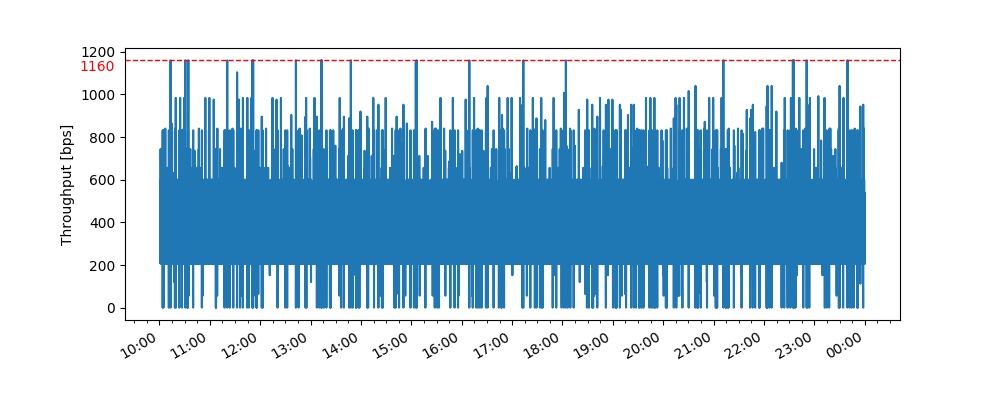
\includegraphics[width=.5\textwidth]{03-tp-simul}
    % \caption{RS485 datarates in simulation of heavy data traffic}
    % \label{fig:heavySimulation}
% \end{figure}

% This test simulated the transmission of more than 190~000 commands from 300 sensor nodes every 5 minutes simultaneously for 12 hours time period. The highest datarate achieved during simulation is 1160~bps, Fig \ref{fig:heavySimulation} red dashed line.

%!!! Tady to mozna chce frekvencni analyzu GW, at vis, jak jsou dlouhe pakety, pak nemusis hadat, nebo napis, ze max. delka je 19 bytů.

%Considering the worst case, ie packets with length of 40 Bytes, we have analytically calculated the maximum number of sensors a network can transmit based on the network transmission rate.

%\textbf{!!! Limit RS485: up to 32 transceivers on the serial bus !!! My vsak mame senzory pres LoRa ...Jo, ale to je fyzicky, to splnujeme, mame jich 13 :-)}
%datasheet: https://www.sparkfun.com/datasheets/Components/General/sp3485CN-LTR.pdf

%Space for peaks 10\% --> maximum packet rate is 324 pps
%Data measured in testing procedure shows Fig.

%\begin{table}[h]
%\centering
%\footnotesize
%\caption{Simple analytics of measured data}
%\begin{tabular}{lr}
%\textbf{Packet length} & \textbf{Bytes} \\ \hline
%Minimum   &   7 B     \\
%Maximum   &  40 B     \\
%mean      &   7,51 B  \\
%Median    &   7 B     \\
%\end{tabular}
%\label{tab: simple-analytics}
%\end{table}


%---
% tabulka, rezervy 10%, 30% ...
% Zjistit kolik sensoru muze byt na sbernici 485.
% popis os co  je co
